\documentclass{article}

\usepackage{fancyhdr}
\usepackage{extramarks}
\usepackage{amsmath}
\usepackage{amsthm}
\usepackage{amsfonts}
\usepackage{tikz}
\usepackage[plain]{algorithm}
\usepackage{algpseudocode}
\usepackage{color}
\usepackage{listings}
\usepackage{fontspec}

\setmainfont{BemboStd}
\setmonofont{Menlo}
\newfontfamily\menlo{Menlo}
\lstset{
    columns=fixed,       
    numbers=left,                                        % 在左侧显示行号
    numberstyle=\tiny\color{gray},                       % 设定行号格式
    frame=none,                                          % 不显示背景边框
    backgroundcolor=\color[RGB]{245,245,244},            % 设定背景颜色
    keywordstyle=\color[RGB]{40,40,255},                 % 设定关键字颜色
    numberstyle=\footnotesize\color{darkgray},           
    commentstyle=\small\menlo\color[RGB]{0,96,96},                % 设置代码注释的格式
    stringstyle=\rmfamily\slshape\color[RGB]{128,0,0},   % 设置字符串格式
    showstringspaces=true,                              % 不显示字符串中的空格
    numberstyle=\small\menlo,
    basicstyle=\small\menlo,
    breaklines=true,
}

% \lstset{
%     language=Octave,                % the language of the code
%     basicstyle=\footnotesize,           % the size of the fonts that are used for the code
%     numbers=left,                   % where to put the line-numbers
%     numberstyle=\tiny\color{gray},  % the style that is used for the line-numbers
%     stepnumber=1,                   % the step between two line-numbers. If it's 1, each line 
%                                     % will be numbered
%     numbersep=5pt,                  % how far the line-numbers are from the code
%     backgroundcolor=\color{white},      % choose the background color. You must add \usepackage{color}
%     showspaces=false,               % show spaces adding particular underscores
%     showstringspaces=false,         % underline spaces within strings
%     showtabs=false,                 % show tabs within strings adding particular underscores
%     frame=single,                   % adds a frame around the code
%     rulecolor=\color{black},        % if not set, the frame-color may be changed on line-breaks within not-black text (e.g. commens (green here))
%     tabsize=2,                      % sets default tabsize to 2 spaces
%     captionpos=b,                   % sets the caption-position to bottom
%     breaklines=true,                % sets automatic line breaking
%     breakatwhitespace=false,        % sets if automatic breaks should only happen at whitespace
%     title=\lstname,                 % show the filename of files included with \lstinputlisting;
%                                     % also try caption instead of title
%     keywordstyle=\color{blue},          % keyword style
%     commentstyle=\color{dkgreen},       % comment style
%     stringstyle=\color{mauve},         % string literal style
%     escapeinside={\%*}{*)},            % if you want to add LaTeX within your code
%     morekeywords={*,...}               % if you want to add more keywords to the set
% }

\usetikzlibrary{automata,positioning}

%
% Basic Document Settings
%
%%% page layout
\topmargin=-0.45in
\evensidemargin=0in
\oddsidemargin=0in
\textwidth=6.5in
\textheight=9.0in
\headsep=0.25in

\linespread{1.1}    %%% line spacing

\definecolor{ustcblue}{cmyk}{1,0.8,0,0}

\pagestyle{fancy}
\lhead{\hmwkAuthorName}
\chead{\hmwkClass\ (\hmwkClassInstructor): \hmwkTitle}
\rhead{}
\lfoot{}
\cfoot{\thepage}

\renewcommand\headrulewidth{0.4pt}
\renewcommand\footrulewidth{0.4pt}

\setlength\parindent{0pt}

%
% Create Problem Sections
%

\newcommand{\enterProblemHeader}[1]{
    \nobreak\extramarks{}{Problem \arabic{#1} continued on next page\ldots}\nobreak{}
    \nobreak\extramarks{Problem \arabic{#1} (continued)}{Problem \arabic{#1} continued on next page\ldots}\nobreak{}
}

\newcommand{\exitProblemHeader}[1]{
    \nobreak\extramarks{Problem \arabic{#1} (continued)}{Problem \arabic{#1} continued on next page\ldots}\nobreak{}
    \stepcounter{#1}
    \nobreak\extramarks{Problem \arabic{#1}}{}\nobreak{}
}

\setcounter{secnumdepth}{0}
\newcounter{partCounter}
\newcounter{homeworkProblemCounter}
\setcounter{homeworkProblemCounter}{1}
\nobreak\extramarks{Problem \arabic{homeworkProblemCounter}}{}\nobreak{}

%
% Homework Problem Environment
%
% This environment takes an optional argument. When given, it will adjust the
% problem counter. This is useful for when the problems given for your
% assignment aren't sequential. See the last 3 problems of this template for an
% example.
%
\newenvironment{homeworkProblem}[1][-1]{
    \ifnum#1>0
        \setcounter{homeworkProblemCounter}{#1}
    \fi
    \subsection{Exercise \arabic{homeworkProblemCounter}}
    \setcounter{partCounter}{1}
    \enterProblemHeader{homeworkProblemCounter}
}{
    \exitProblemHeader{homeworkProblemCounter}
}

%
% Homework Details
%   - Title
%   - Due date
%   - Class
%   - Section/Time
%   - Instructor
%   - Author
%

\newcommand{\hmwkTitle}{Homework\ \#4}
\newcommand{\hmwkDueDate}{\today}
\newcommand{\hmwkClass}{Inversion}
\newcommand{\hmwkClassInstructor}{Professor H. Yao \& H. Zhang}
\newcommand{\hmwkAuthorName}{\textbf{Jintao Li}}
\newcommand{\hmwkAuthorID}{\textbf{SA20007037}}
\newcommand{\hmwkAuthoremail}{\textbf{E-mail: lijintao@mail.ustc.edu.cn}}

%
% Title Page
%

% \title{
%     \vspace{2in}
%     \textbf{\hmwkClass:\ \hmwkTitle}\\
%     \normalsize\vspace{0.2in}\large{\hmwkDueDate}\\
%     \vspace{0.2in}\large{\textit{\hmwkClassInstructor}}
%     \vspace{3in}
% }

% \author{\hmwkAuthorName \\
% \hmwkAuthorID}
% \date{}

\renewcommand{\part}[1]{\textbf{ \\ (\alph{partCounter})  }\stepcounter{partCounter} }

%
% Various Helper Commands
%

% Useful for algorithms
\newcommand{\alg}[1]{\textsc{\bfseries \footnotesize #1}}

% For derivatives
\newcommand{\deriv}[1]{\frac{\mathrm{d}}{\mathrm{d}x} (#1)}

% For partial derivatives
\newcommand{\pderiv}[2]{\frac{\partial}{\partial #1} (#2)}

% Integral dx
\newcommand{\dx}{\mathrm{d}x}

% Alias for the Solution section header
\newcommand{\solution}{\textbf{\large \\ Solution: \\}}

% Probability commands: Expectation, Variance, Covariance, Bias
\newcommand{\E}{\mathrm{E}}
\newcommand{\Var}{\mathrm{Var}}
\newcommand{\Cov}{\mathrm{Cov}}
\newcommand{\Bias}{\mathrm{Bias}}

%
\newcommand{\mb}[1]{\mathbf{#1}}
\newcommand{\mt}[1]{\begin{bmatrix}#1\end{bmatrix}}

\begin{document}

\begin{titlepage}

\begin{center}

\textcolor{ustcblue}{\includegraphics[width=0.25\textwidth]{./ustc_logo_fig.pdf} \\ [1cm]}
% Title
{ \Huge \bfseries \hmwkClass\ \hmwkTitle}\\[1cm]

\large \textbf{\hmwkClassInstructor} \\ [5cm]

\large \hmwkAuthorName \\ [0.25cm]
\large \hmwkAuthorID \\ [0.25cm]
\large \hmwkAuthoremail
\vfill
% Bottom of the page
{\large \today}

\end{center}

\end{titlepage}

\begin{center}
\section{Chapter 3}
\end{center}

\begin{homeworkProblem}[2]
Another resolution test commonly performed in tomography studies is a 
\textbf{checkerboard test}, which consists of using a test model composed 
of alternating positive and negative perturbations. Perform a checkerboard 
test on the tomography problem in Example 3.1 using the test model, 
\begin{equation}
    \mb{m}_{true} = \mt{-1 & 1 & -1 \\ 1 & -1 & 1 \\ -1 & 1 & -1}
\end{equation}
Evaluate the difference between the true (checkerboard) model and the 
recovered model in your test, and interpret the pattern of differences. 
Are any block values recovered exactly? If so, does this imply perfect 
resolution for these model parameters?

\solution

\textbf{matlab code}
\begin{lstlisting}[language={matlab}]
clear;clc;close all;

a = ones(5, 1)
% ls tme
\end{lstlisting}



\end{homeworkProblem}

\begin{homeworkProblem}[4]
A large north-south by east-west–oriented, nearly square plan view, 
sandstone quarry block (16 m by 16 m) with a bulk compressional wave 
seismic velocity of approximately 3000 m/s is suspected of harboring 
higher-velocity dinosaur remains. An ultrasonic tomography scan is 
performed in a horizontal plane bisecting the boulder, producing a data 
set consisting of 16 E$\rightarrow$W, 16 N$\rightarrow$S, 31 NE$\rightarrow$SW, 
and 31 NW$\rightarrow$SE travel times 
(see Figure~\ref{fig:pro}). The travel time data (units of s) have statistically 
independent errors, and the travel time contribution for a uniform background
model (with a velocity of 3000 m/s) has been subtracted from each travel time
measurement.\\

The MATLAB data files that you will need to load containing the travel time data
follow: \textbf{rowscan.mat}, \textbf{colscan.mat}, \textbf{diag1scan.mat}, 
and \textbf{diag2scan.mat}. The standard deviations of all data measurements 
are $1.5 × 10^{-5}$ s. Because the travel time contributions for a uniform 
background model (with a velocity of 3000 m/s) have been subtracted from each 
travel time measurement, you will be solving for slowness and velocity 
perturbations relative to a uniform slowness model of 1/3000 s/m. Use a 
row-by-row mapping between the slowness grid and the model vector 
(e.g., Example 1.12). The row format of each data file is 
$(x_1, \gamma_1, x_2, \gamma_2, t)$ where the starting
point coordinate of each source is $(x_1, \gamma_1)$, the end point coordinate 
is $(x_2, \gamma_2)$, and the travel time along a ray path between the 
source and receiver points is a path integral (in seconds).

\begin{figure}[htb]
    \centering
    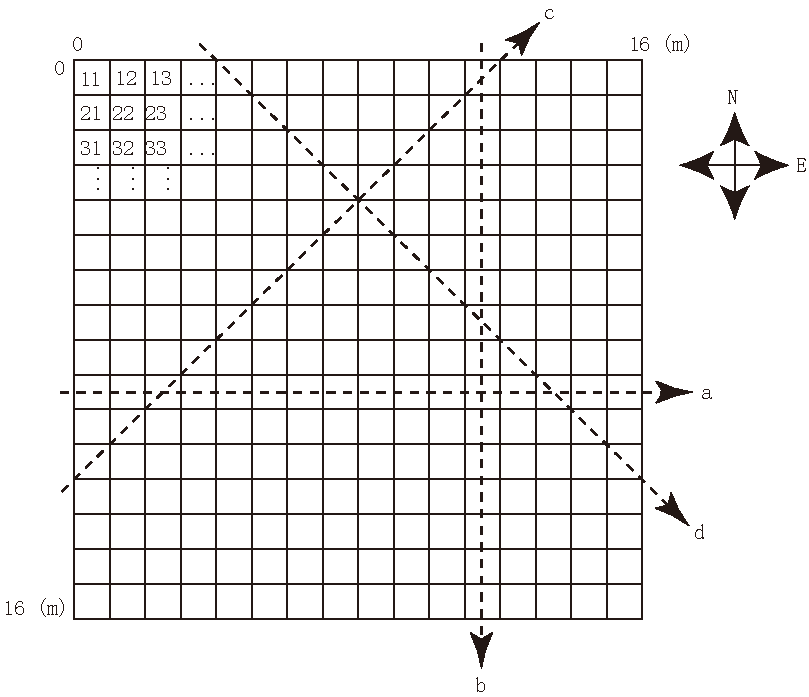
\includegraphics[width=6in, keepaspectratio]{hw4/pro.pdf}
    \caption{Tomography exercise, showing block discretization, 
    block numbering convention, and
    representative ray paths going east-west (a), north-south (b), 
    southwest-northeast (c), and northwestsoutheast (d).}
    \label{fig:pro}
\end{figure}

Parameterize the slowness structure in the plane of the survey by dividing the
boulder into a $16\times16$ grid of 256 1-m-square, north-by-east blocks and construct
a linear system for the forward problem (Figure 3.29). Assume that the ray paths
through each homogeneous block can be represented by straight lines, so that the
travel time expression is
\begin{equation}
    \begin{aligned}
    t &=\int_{\ell} s(\mathbf{x}) d \ell \\
    &=\sum_{\text {blocks }} s_{\text {block }} \cdot \Delta l_{\text {block }}
    \end{aligned}
\end{equation}
where $\Delta l_{block}$ is 1 m for the row and column scans and $\sqrt{2}$ m for 
the diagonal scans. \\

Use the SVD to find a minimum-length/least squares solution, $\mathbf{m}_{\dagger}$, 
for the 256 block slowness perturbations that fit the data as exactly as possible. 
Perform two inversions in this manner: \\
1. Use the row and column scans only. \\
2. Use the complete data set. \\
For each inversion: \\

\part

Note the rank of your \textbf{G} matrix relating the data and model.

\part

State and discuss the general solution and/or data fit significance of the elements
and dimensions of the data and model null spaces. Plot and interpret an element
of each space and contour or otherwise display a nonzero model that fits the
trivial data set $\mb{Gm} = \mb{d} = \mb{0}$ exactly.

\part

Note whether there are any model parameters that have perfect resolution.

\part

Produce a 16 by 16 element contour or other plot of your slowness perturbation
model, displaying the maximum and minimum slowness perturbations in the
title of each plot. Interpret any internal structures geometrically and in terms of
seismic velocity (in m/s).

\part

Show the model resolution by contouring or otherwise displaying the 256
diagonal elements of the model resolution matrix, reshaped into an appropriate
16 by 16 grid.

\part

Describe how one could use solutions to $\mb{Gm} = \mb{d} = \mb{0}$ to 
demonstrate that very
rough models exist that will fit any data set just as well as a generalized inverse
model. Show one such wild model.


\end{homeworkProblem}


\end{document}
